\section{Results and Discussions}
\label{sec:results}
The following section presents and discusses the results for this project namely the ploy length parameter and  bending stiffness of the boom derived with respect to change in the clamp width. These results would be used to explain the results obtained in the bending and flattening cycles of the booms with different clamp widths, one example of which is shown in figure \ref{fig:sequence}. 
%seq for deformation. 
\begin{figure}[!hbt]
\begin{subfigure}{.5\linewidth}
\centering
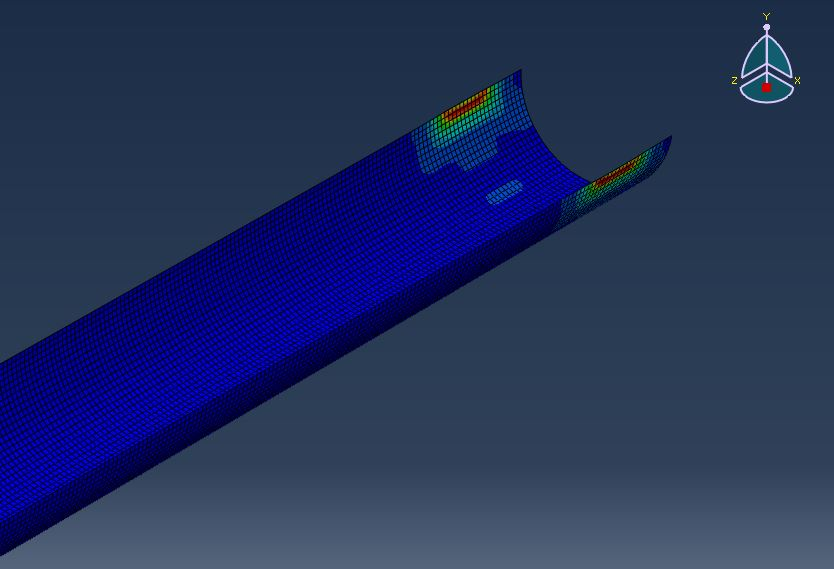
\includegraphics[height=4.5cm]{images/1.JPG}
\caption{}
\label{fig:sub1}
\end{subfigure}%
\begin{subfigure}{.5\linewidth}
\centering
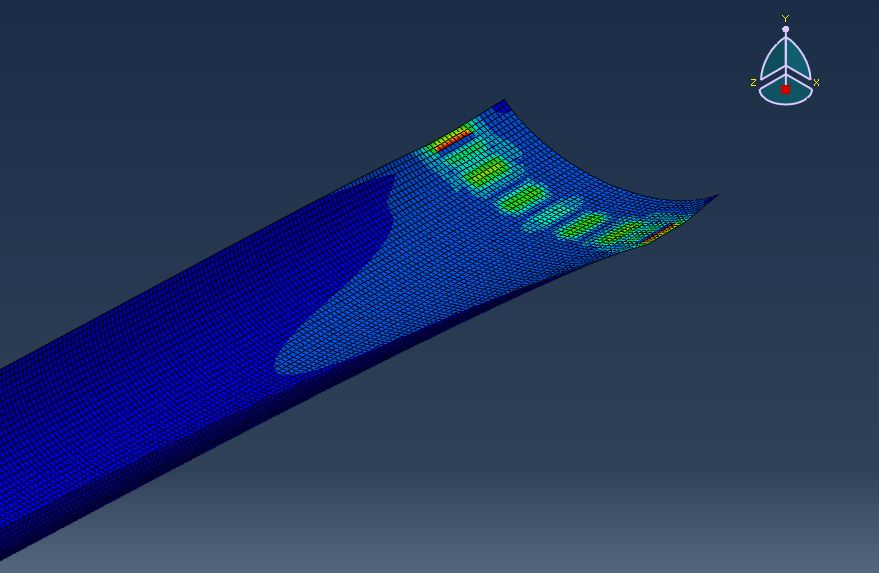
\includegraphics[height=4.5cm]{images/3.JPG}
\caption{}
\label{fig:sub2}
\end{subfigure}
\begin{subfigure}{.5\linewidth}
\centering
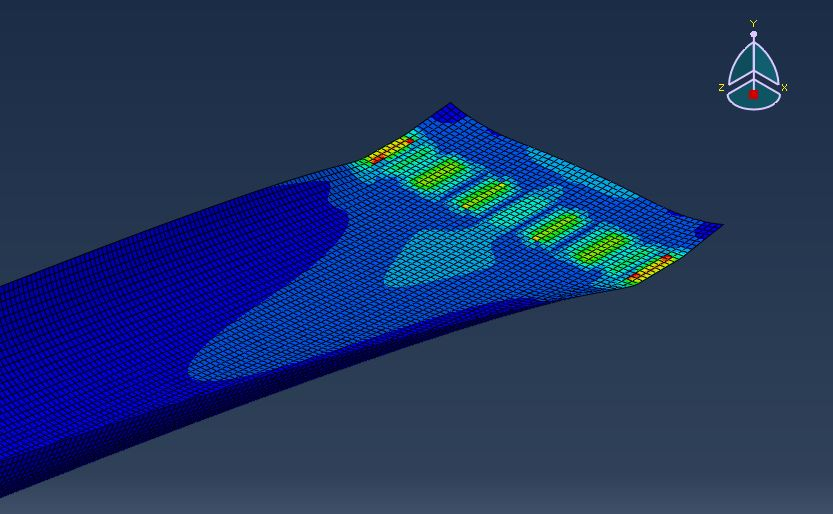
\includegraphics[height=4.5cm]{images/4.JPG}
\caption{}
\label{fig:sub3}
\end{subfigure}
\label{fig:test}
\begin{subfigure}{.5\linewidth}
\centering
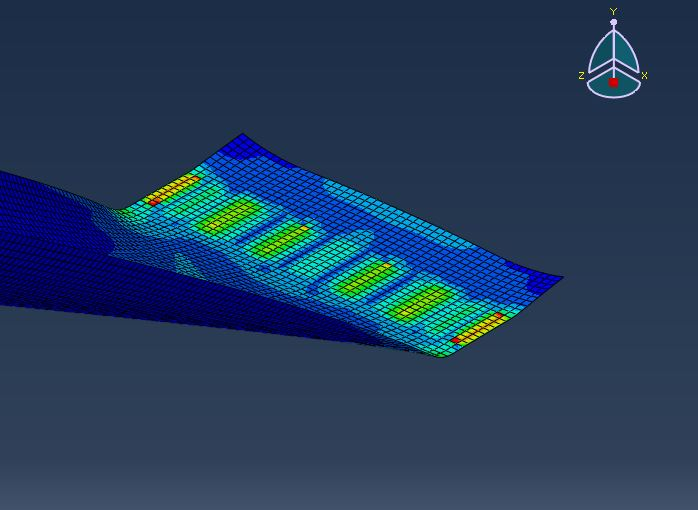
\includegraphics[height=4.5cm]{images/6.JPG}
\caption{}
\label{fig:case24}
\end{subfigure}
\caption{Sequence of flattening of the root and bending of a fully clamped boom in ABAQUS in order (a) to (d)}
\label{fig:sequence}
\end{figure}

\subsection{Lateral displacement}

% need fig 1 before text? or some intro at least? 
Figure \ref{fig:ploy1} shows a plot showing the deformed width of the boom along the length with different clamp widths at the root of the boom. It is observed that the maximum lateral width of the boom increases with an increase in width of the root clamp, which can also be observed in figure \ref{fig:ploydefine}. 

\begin{figure}[!hbt]
    \centering
    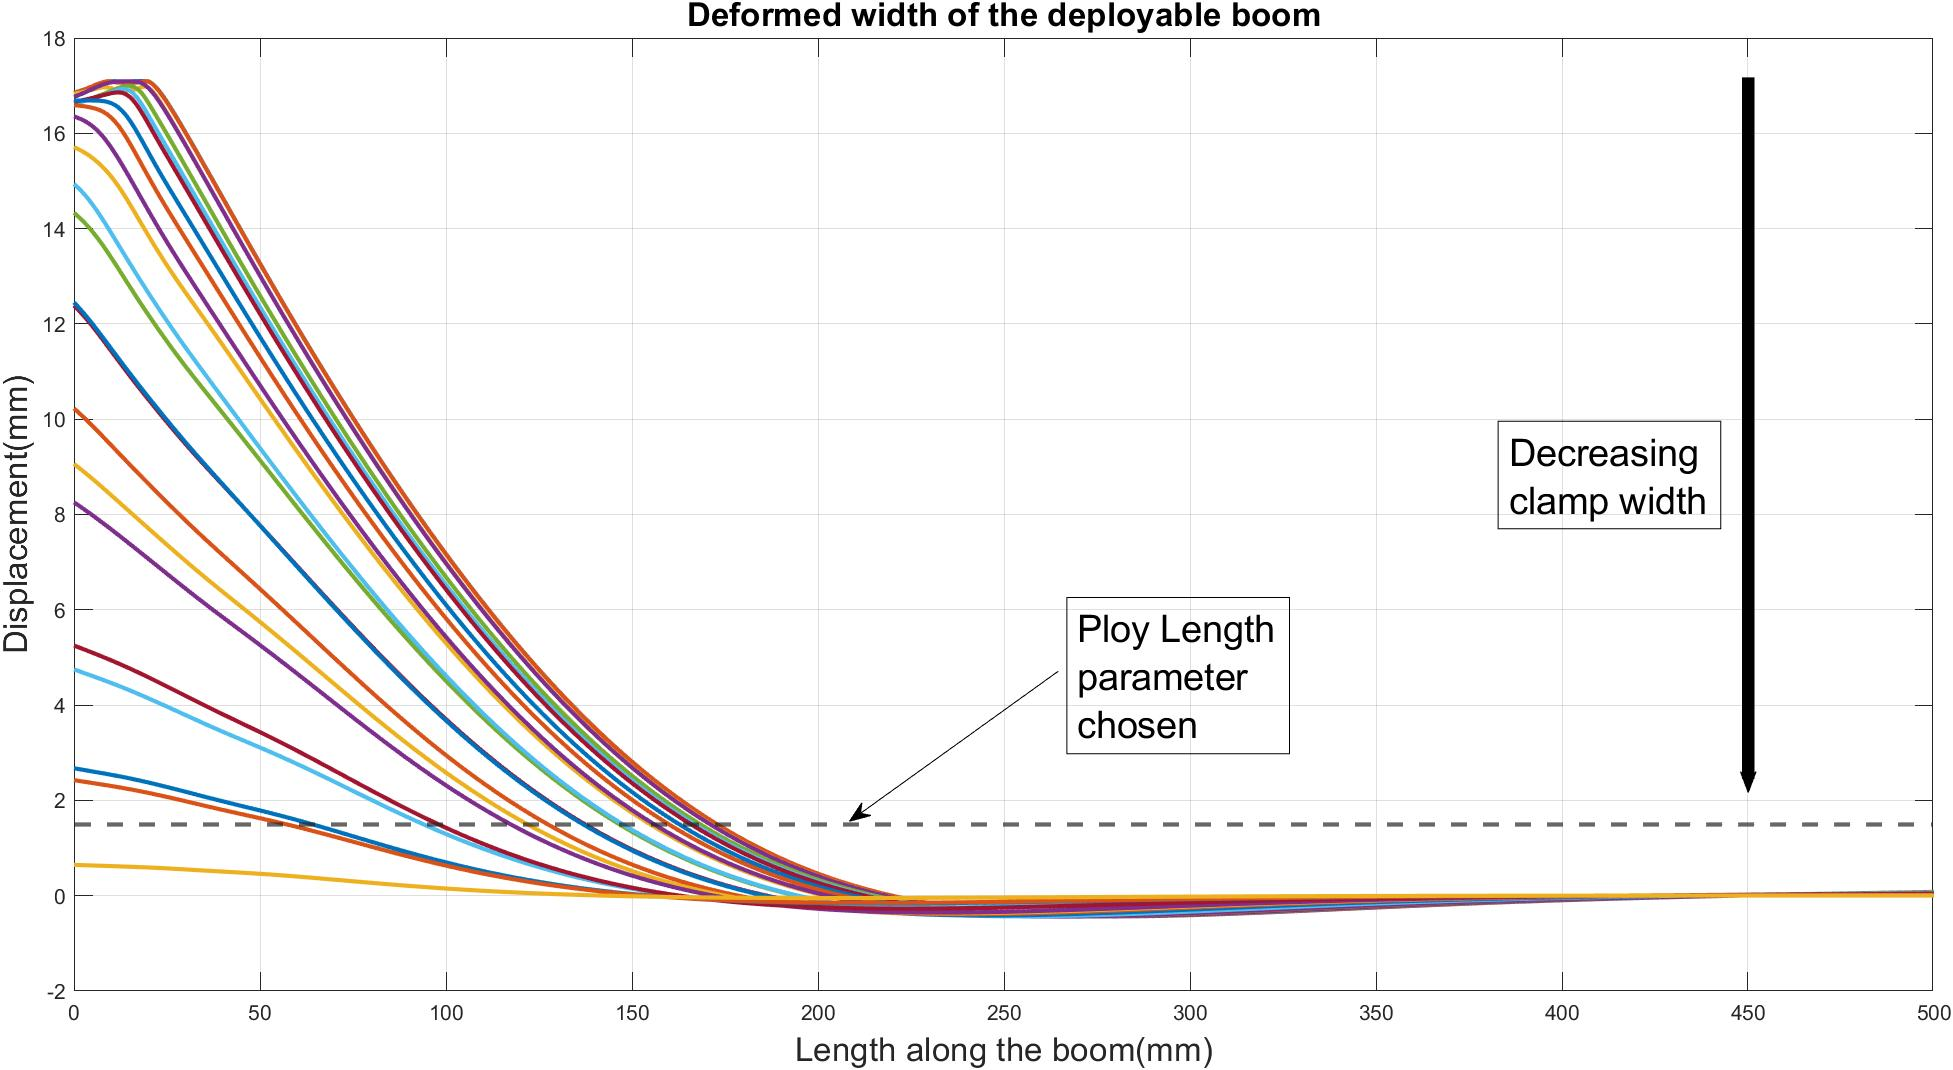
\includegraphics[width=15cm]{images/maxwidth.jpg}
    \caption{Deformed width of boom compared to the length of the boom}
    \label{fig:ploy1}
\end{figure}

Interestingly, it is also observed that the tape bends slightly inwards around the middle of the boom thus giving a negative displacement. However the maximum limit of this negative displacement is nearly constant at -0.44mm. Further, the different cases return to null displacement at nearly the same length. This is shown more clearly in the figure \ref{fig:negdisp}.   

\begin{figure}[!hbt]
    \centering
    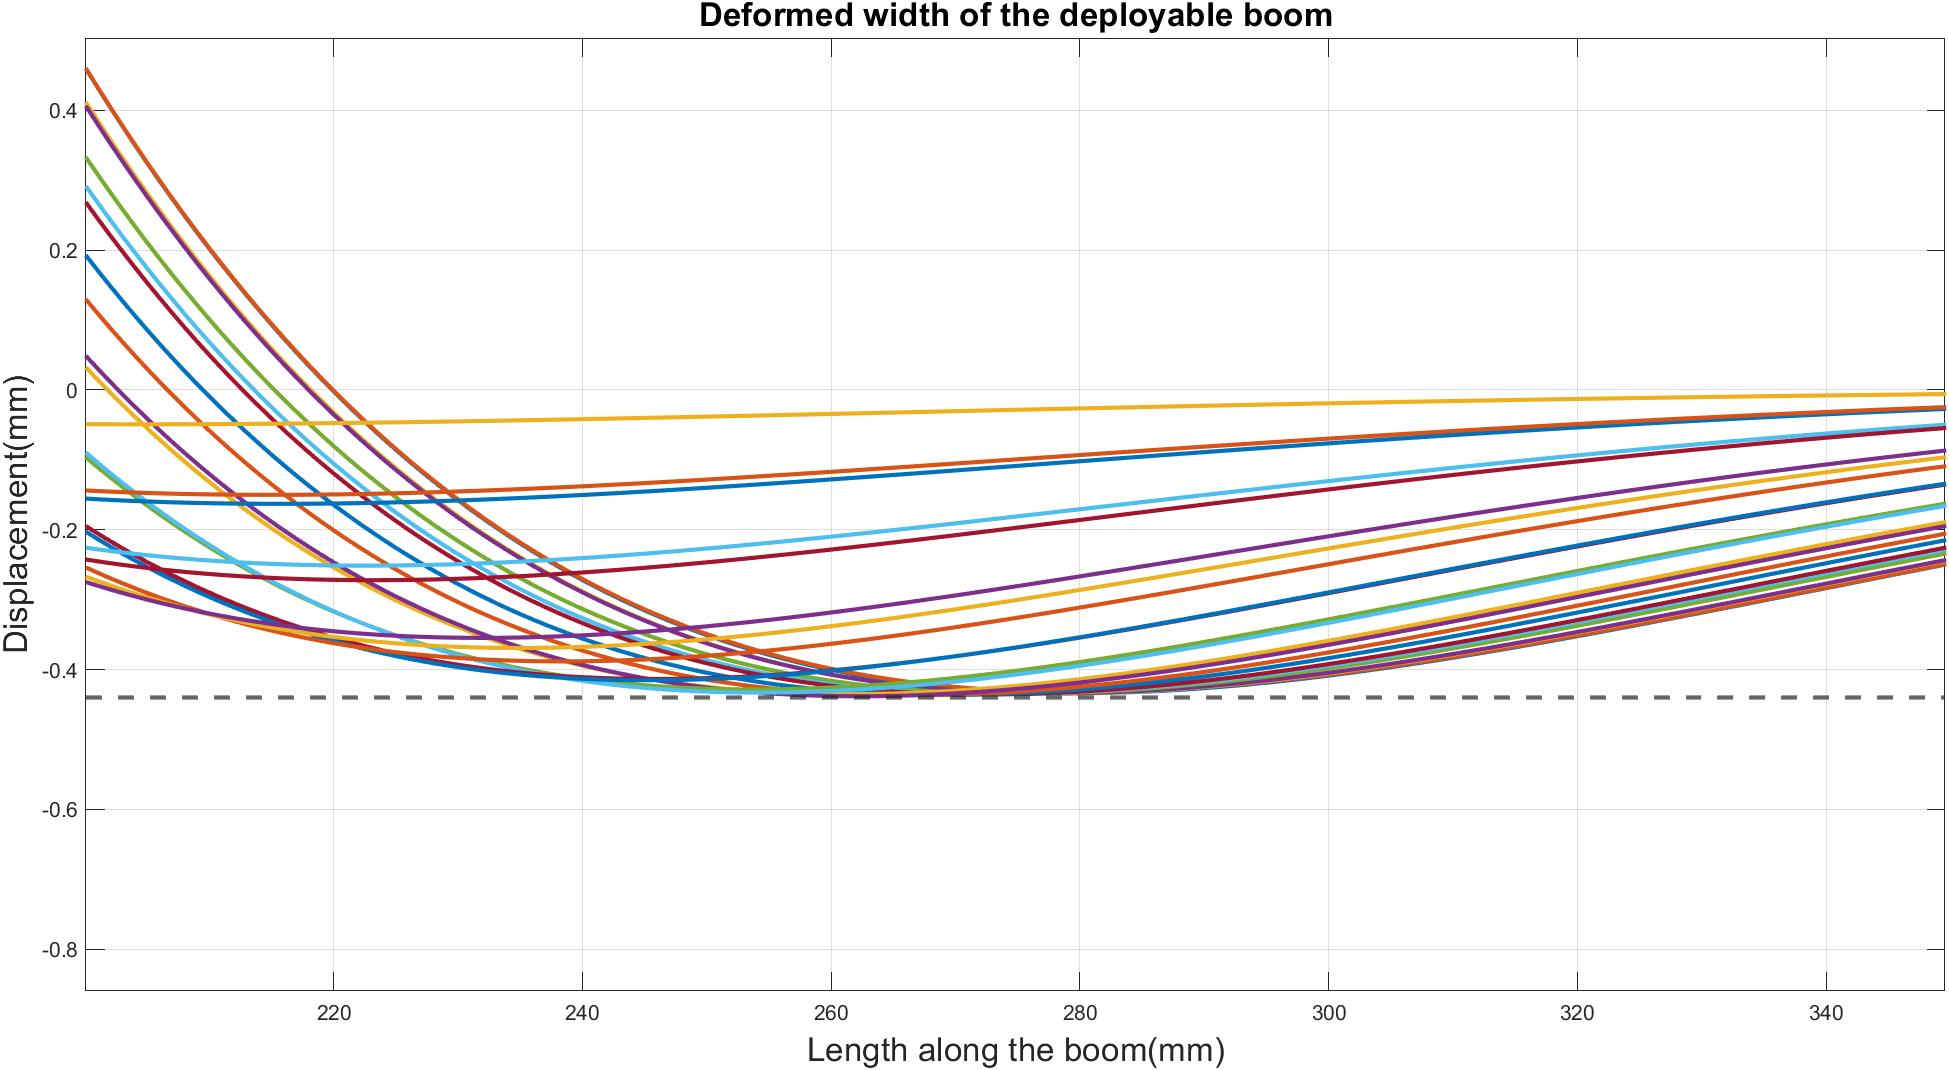
\includegraphics[width=15cm]{images/zoomin.jpg}
    \caption{Negative displacement}
    \label{fig:negdisp}
\end{figure}
\subsection{Ploy length parameter}
Figure \ref{fig:ploydefine} shows the deformed boom once the boundary conditions were applied in FE software ABAQUS. After flattening of the boom, the boom returns to its original curvature further along the distance. The ploy legnth parameter is the distance along the boom from the clamp where it is flattened to where the lateral width of the deformed boom is nearly equal to the lateral width before the deformation. In this paper, it is selected to be 5\% deviation of the undeformed width of the boom. The ploy length is an important result as this later helps in the design of a STEM boom deployer, by allowing for the positioning of guide rollers to ensure smooth deployment of the boom and keeping its alignment shown in figure \ref{fig:guiderollers}. 
\begin{figure}[!hbt]
    \centering
    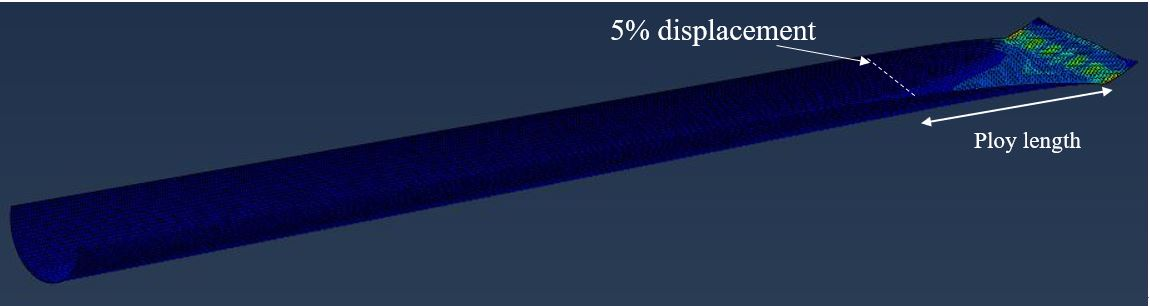
\includegraphics[width=15cm]{images/pic1.JPG}
    \caption{Ploy length}
    \label{fig:ploydefine}
\end{figure}

\begin{figure}[!hbt]
    \centering
    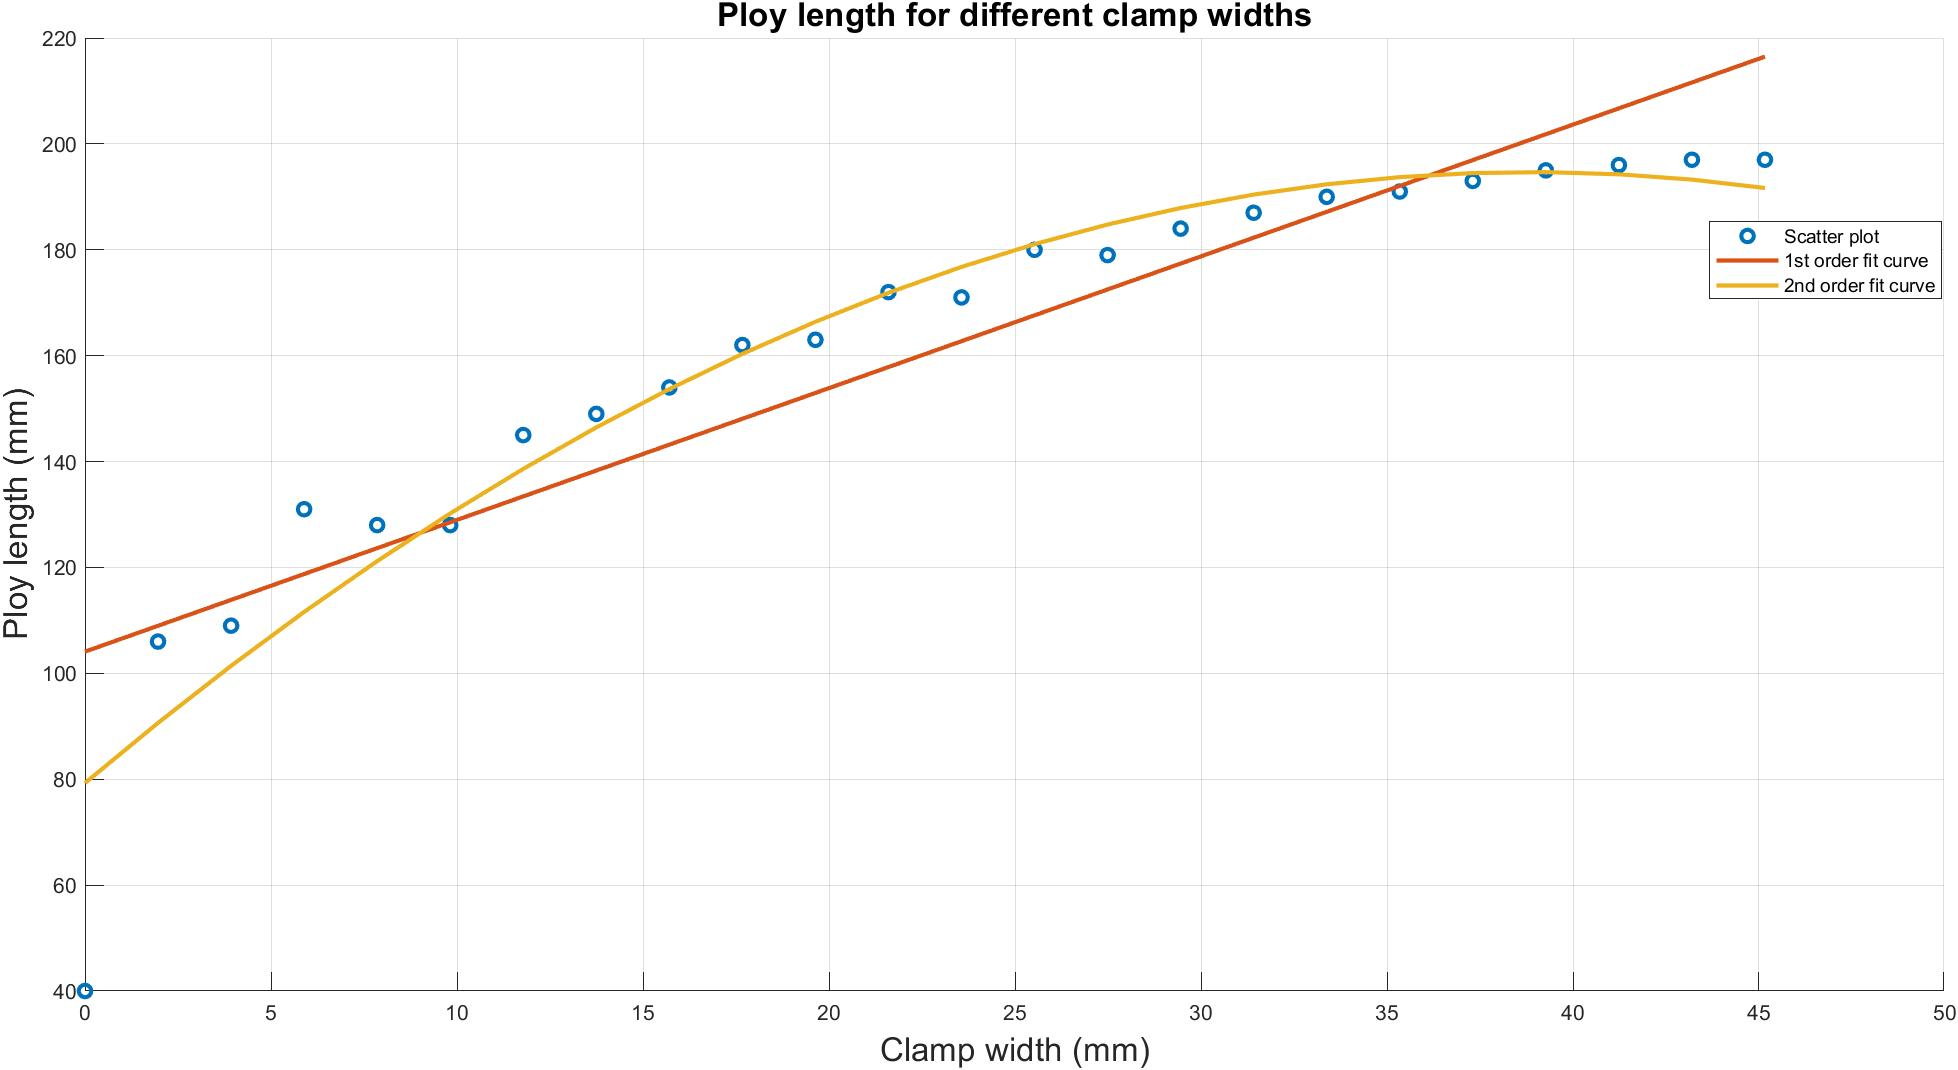
\includegraphics[width=15cm]{images/fitcurve.jpg}
    \caption{Ploy length second order fitted curve}
    \label{fig:fitcurve}
\end{figure}
In figure \ref{fig:fitcurve}, the scatter points are the ploy lengths of the different cases obtained by using the above mentioned ploy length parameter. Figure \ref{fig:fitcurve} shows the fitting of polynomial curves to the data obtained. In the plot a first order and second order equations are compared with regards to their fit with the data, and it is observed that the second order curve is better suited as a relation curve between the width of the clamp and the ploy length. The equations were obtained using MATLAB's polyfit function. The second order fit for the ploy length $L_{\mathrm{ploy}}$ is given by equation \ref{eq:ployfit}
\begin{equation}
    L_{\mathrm{ploy}}=-0.08 \times W^2+5.93 \times W+79.28
    \label{eq:ployfit}
\end{equation}
where $W$ is the width of the clamp area. 
%definition of ploy length 
The definition of this ploy length was chosen to be 5\% deviation of undeformed lateral width of the boom. Reference \cite{Yang2018} fixes the definition for the ploy length to be 5\% deviation in the curvature of the boom, however for the purposes of the report the length parameter is chosen. In this case, a 5\% deviation of the diameter of 30mm is 1.5mm.  A plot comparing different definitions is given in figure \ref{fig:ploydef}, which shows that the different even if a parameter for 10\% or 15\%  was taken, the shape of the plot does not change, validating this paper's parameter selection.  
\begin{figure}[!hbt]
    \centering
    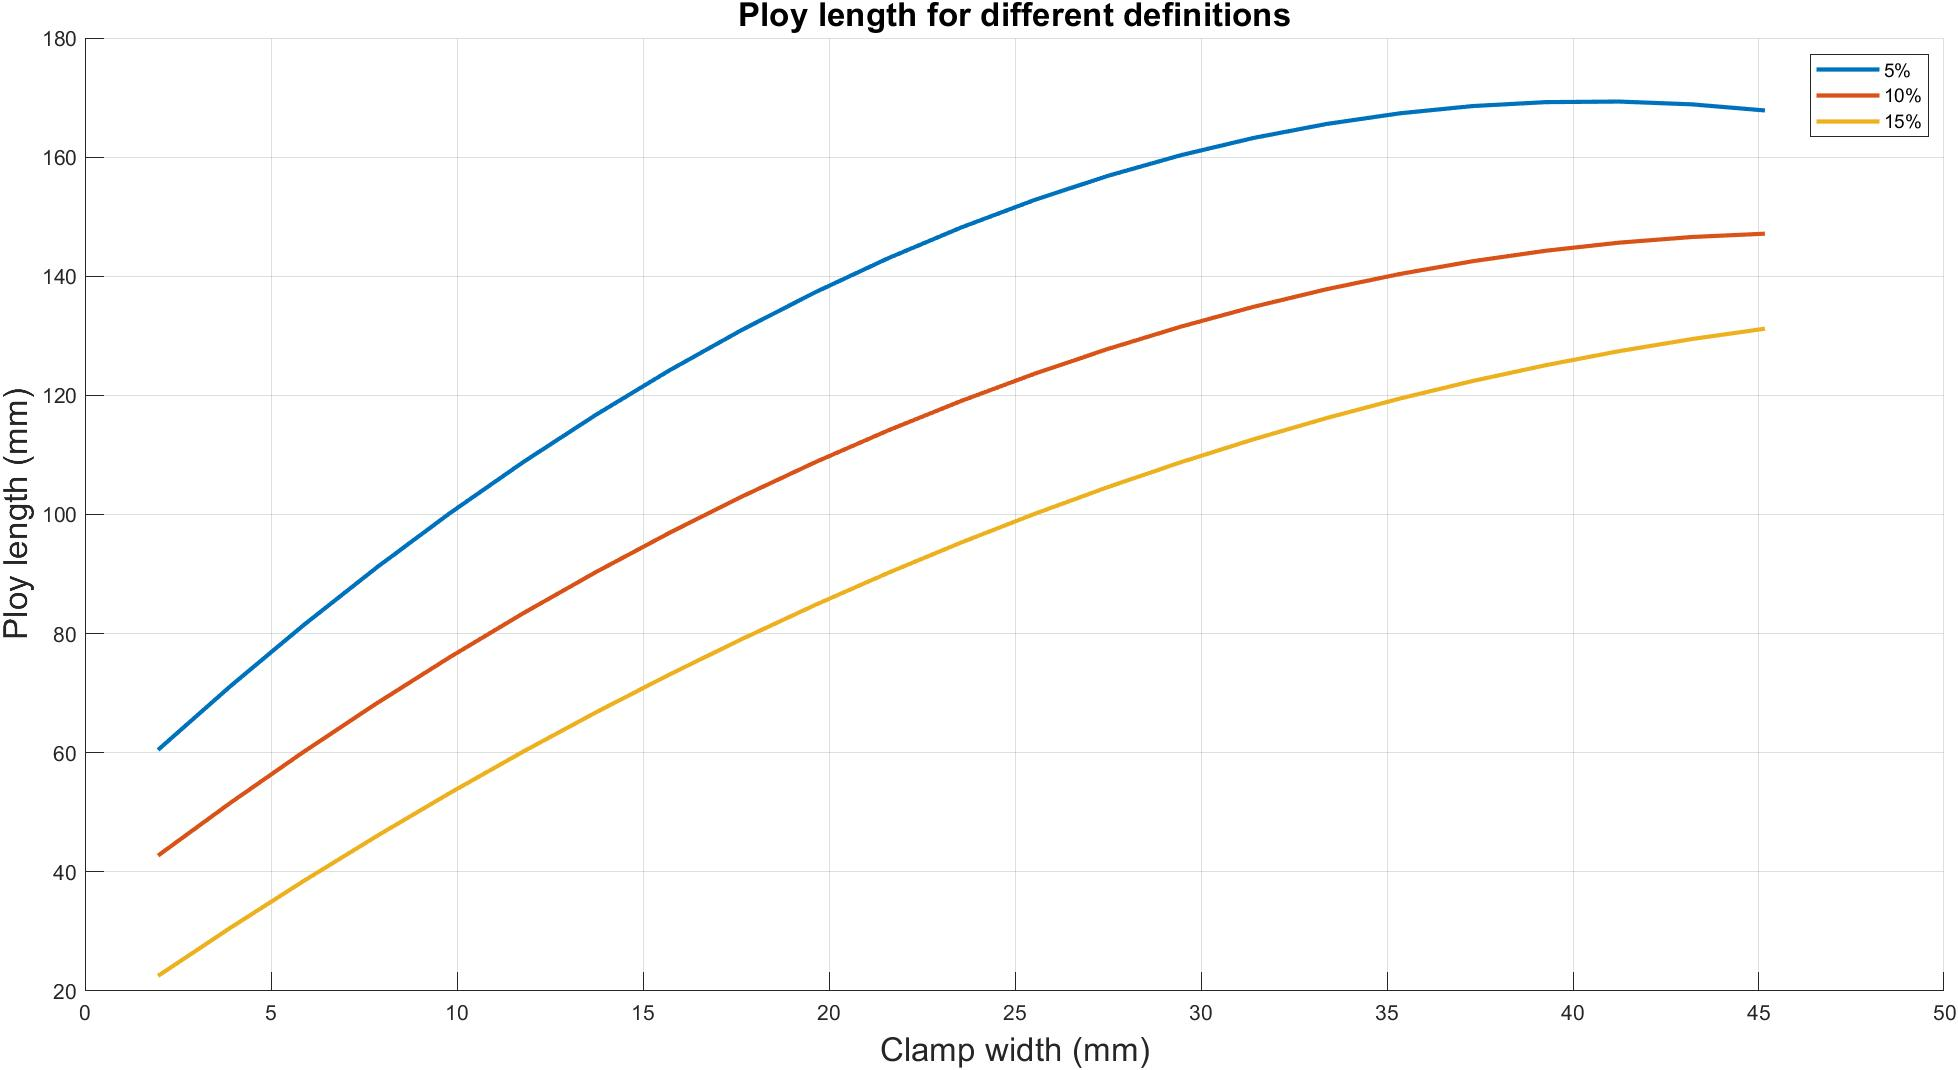
\includegraphics[width=15cm]{images/ploylen_def.jpg}
    \caption{Ploy length plots for different definitions}
    \label{fig:ploydef}
\end{figure}
\subsection{Bending stiffness}
\begin{figure}[!hbt]
    \centering
    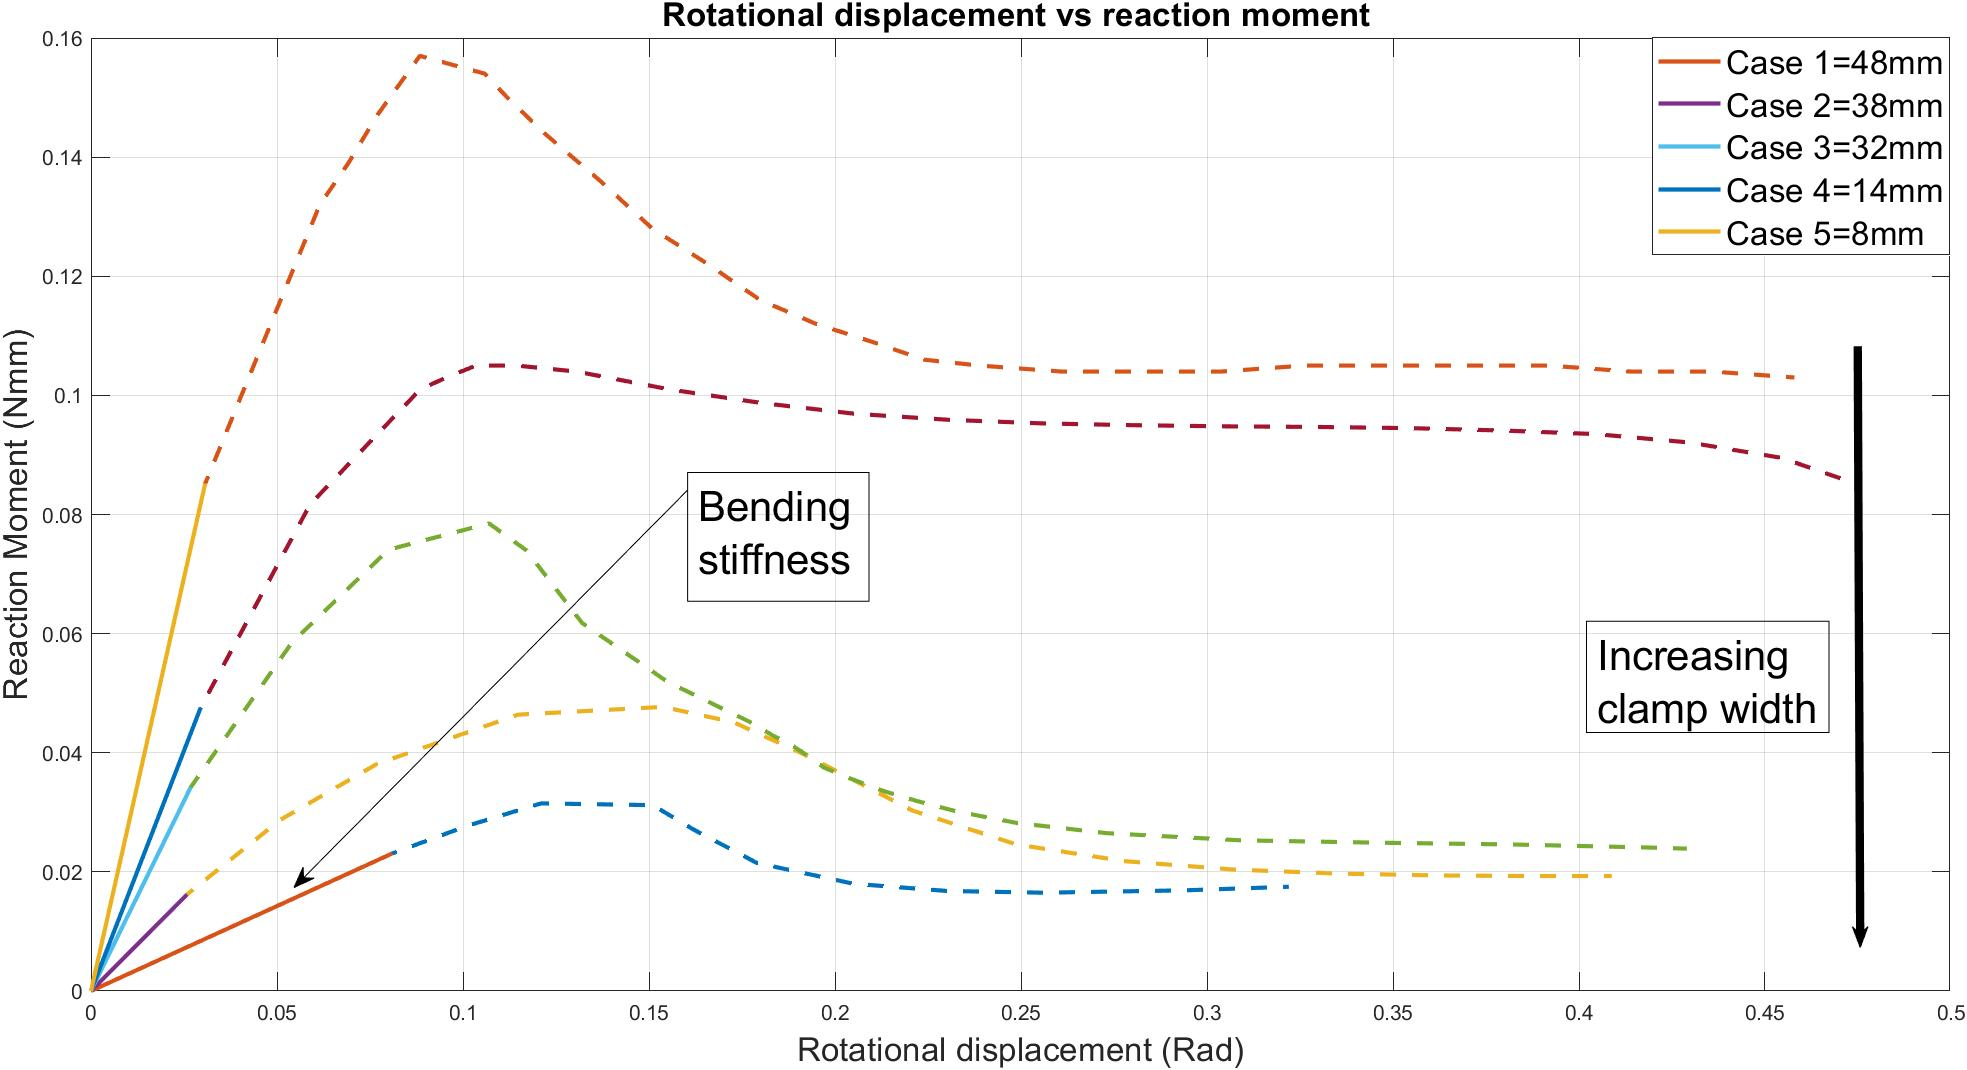
\includegraphics[width=15cm]{images/rotdispupdated.jpg}
    \caption{Rotational displacement plotted against reaction moment for varying clamp widths}
    \label{fig:rotdisp}
\end{figure}
% put a new image without the fitted curve + possibly new data points. 
Figure \ref{fig:rotdisp} shows the relationship between the reaction moment and the rotational displacements for different clamp widths for applied same sense bending. In this plot case 1 is fully encastered whereas case 5 has the least clamp width. The linear slope shown in the plot is used to calculate the bending stiffness of the booms for the different clamp widths in figure \ref{fig:bendstiff}. The curves initially reach a peak maximum reaction moment and thereafter there is a sharp decrease in reaction moment. Once this propagation moment is reached it remains constant for further increase in $\theta$. This is because the boom initially deflects upwards and after reaching the peak moment, it buckles resulting in a sharp decrease in reaction moment \cite{Seffen1999} as can be seen in figure \ref{fig:boom}. This buckling leads to a fold development across the width of the boom as shown in figure \ref{fig:case24} also discussed in the literature review. 
The peak reaction moment and subsequently bending stiffness of the booms increase with a decrease in clamp width. This is because of non-linear fold-support effects on the booms observed in figure \ref{fig:foldint}, which is a plot of peak reaction moments with respect to y/R which is essentially the extent of the fold developed across the boom \cite{Seffen1999}. Comparing figure \ref{fig:case19} which has a clamp width of 38mm and figure \ref{fig:case24} which is fully flat with a clamp width of 48mm, the extent of the fold developed across the boom is different. This is because a narrow clamp has a different transverse curvature to that of the fold. Thus, figure \ref{fig:case19} has a partial fold which results in a higher peak moment for a narrower clamp in figure \ref{fig:rotdisp}. Figure \ref{fig:case24} has a full fold since the boundary condition has the same curvature as that of the fold, and thus its peak moment is lower.
\begin{figure}[!hbt]
     \centering
     \begin{subfigure}[b]{0.4\textwidth}
         \centering
    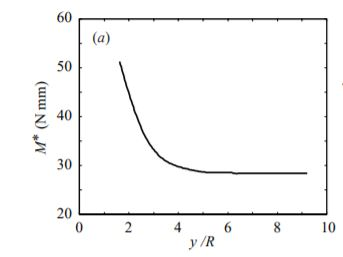
\includegraphics[height=4.5cm]{images/foldinteraction.JPG}
    \caption{Fold interaction with varying y/R from source \cite{Seffen1999}}
    \label{fig:foldint}
     \end{subfigure}
     \hfill
     \begin{subfigure}[b]{0.4\textwidth}
         \centering
    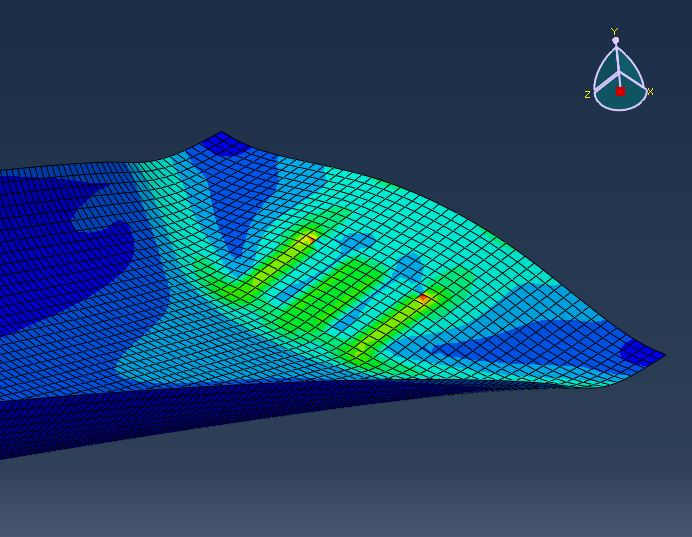
\includegraphics[height=4.5cm]{images/halfwidth.JPG}
     \caption{Fold development in a clamp with narrower width}
  \label{fig:case19}
     \end{subfigure}
     \caption{Fold support interaction}
\end{figure}
%so how does fold influence the bending moment?
A fully developed fold across the boom causes a decrease in energy which results in lowering of the reaction moment and consequently the bending stiffness. Mansfield et. al. have developed a theory for same sense bending based on Calladine's shell theory \cite{calladine_1983} analyzing a strip of constant thickness on a cylinder to be taken as a tape spring. More details are shown in figure \ref{fig:mansfield} in appendix. According to this theory, the equation for longitudinal bending moment, $m_{yz}$ is given by equation \ref{eq:mansfield} from reference \cite{Seffen1999}. 
\begin{equation}
    m_{yz}=D\Bigg[\nu(\dv[2]{u}{z}+\frac{1}{R})+(\frac{1}{r_1})\Bigg]
    \label{eq:mansfield}
\end{equation}
Where, $D=\frac{Et^3}{12(1-\nu^2)}$, $\dv[2]{u}{z}$ is the differential of the height of the tapespring and $\frac{1}{r_1}$ is local curvature at a point. Due to the formation of a flat fold the factor, $\dv[2]{u}{z}=0$ hence there is a significant reduction in bending moment compared to a constrained boom. 
%propogating moment
It is also seen that the propagating moments are different for different clamped widths. It is plausible that due to the above mentioned fold-support interactions the propagating moments increase for a decrease in clamp width. 
\begin{figure}[!hbt]
    \centering
    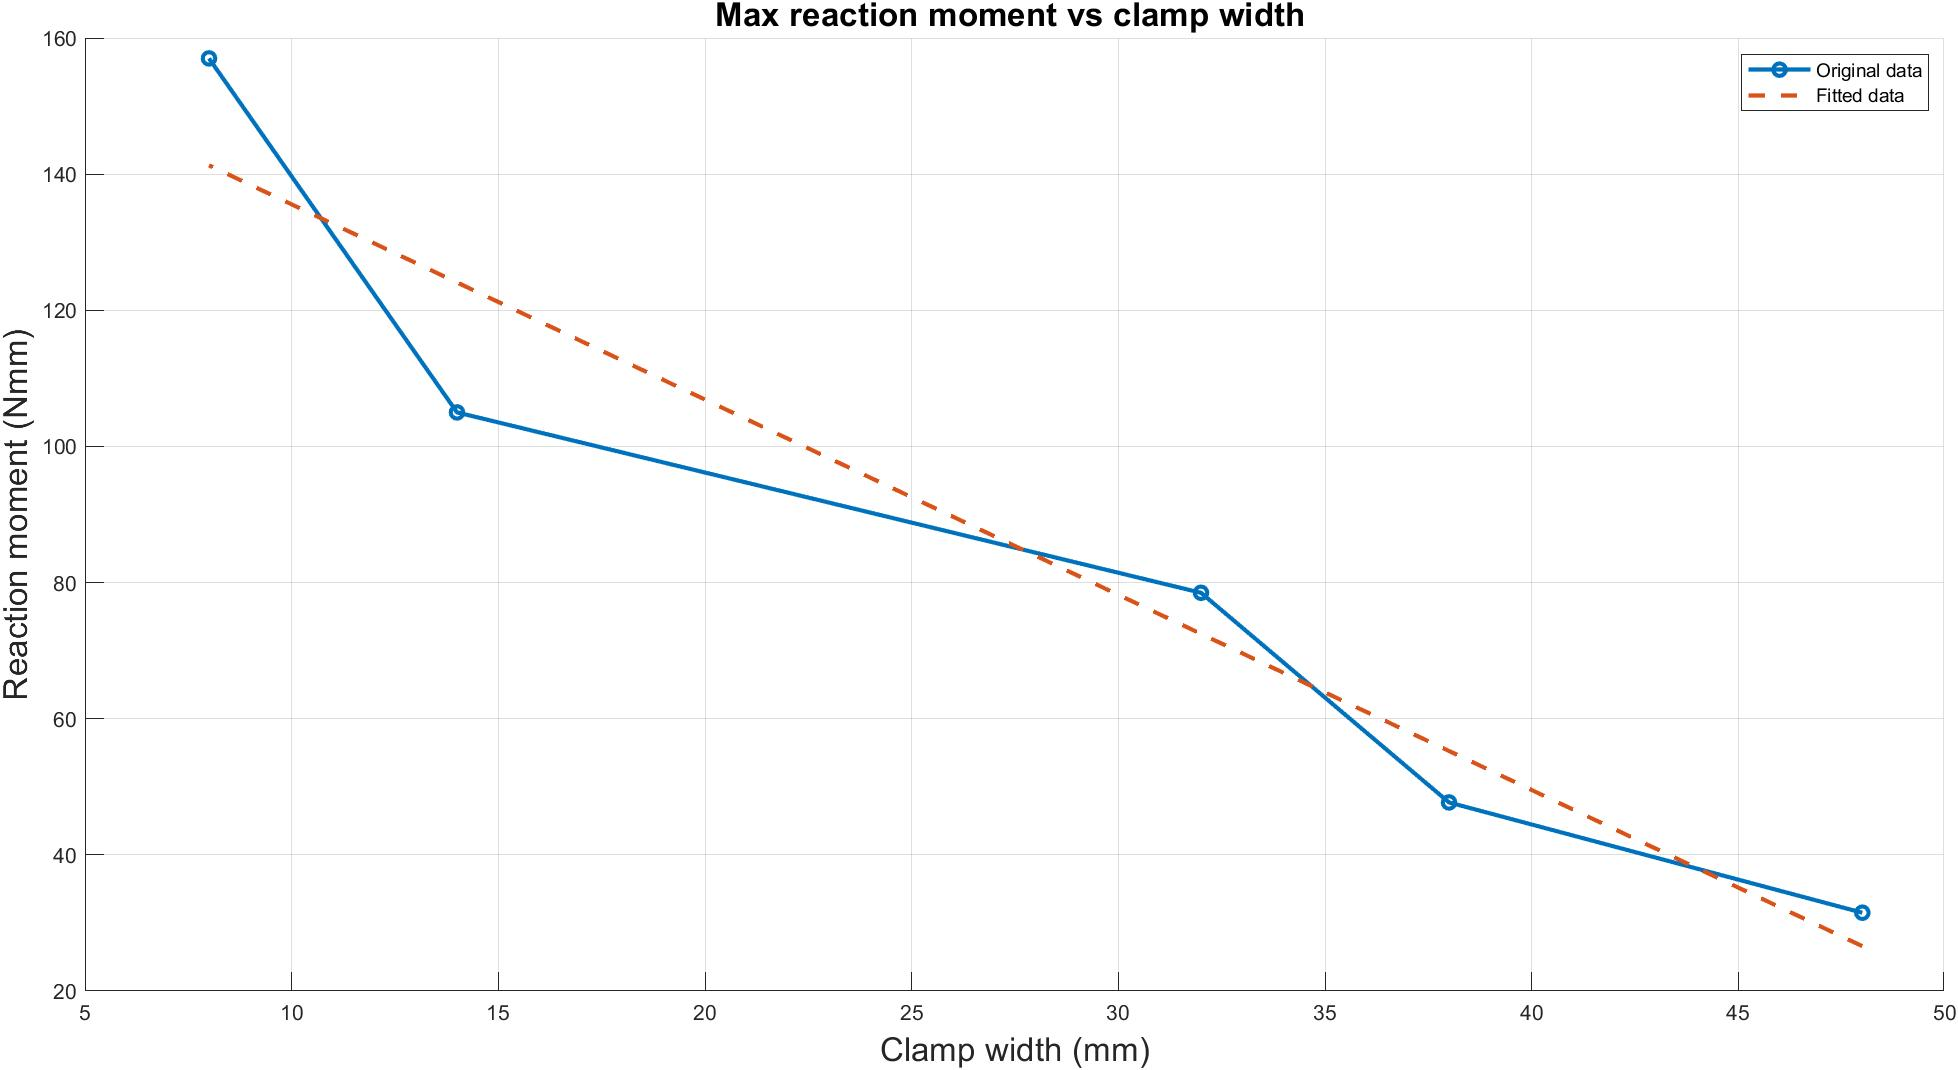
\includegraphics[width=15cm]{images/maxRM.jpg}
    \caption{Fitted curve for the plot between the maximum reaction moment and clamp width}
    \label{fig:maxRM}
\end{figure}
The following plot shows the relationship between maximum reaction moment for differing clamp widths. The correlation factor of the two variables is given by -0.9624 indicating a strong linear negative correlation between the two variables. Thus when the width increases the rotational moment decreases and vice versa. A linear curve is fitted across the data to give the following plot with the following equation, where $R_{\mathrm{max}}$ is the maximum reaction moment and W is the width of the clamp width.   
 \begin{equation}
     R_{\mathrm{max}}=-2.87\times W+ 164.24
     \label{eq:maxRM}
 \end{equation}
The table with the points above is given in the appendix. 
\begin{figure}[!hbt]
    \centering
    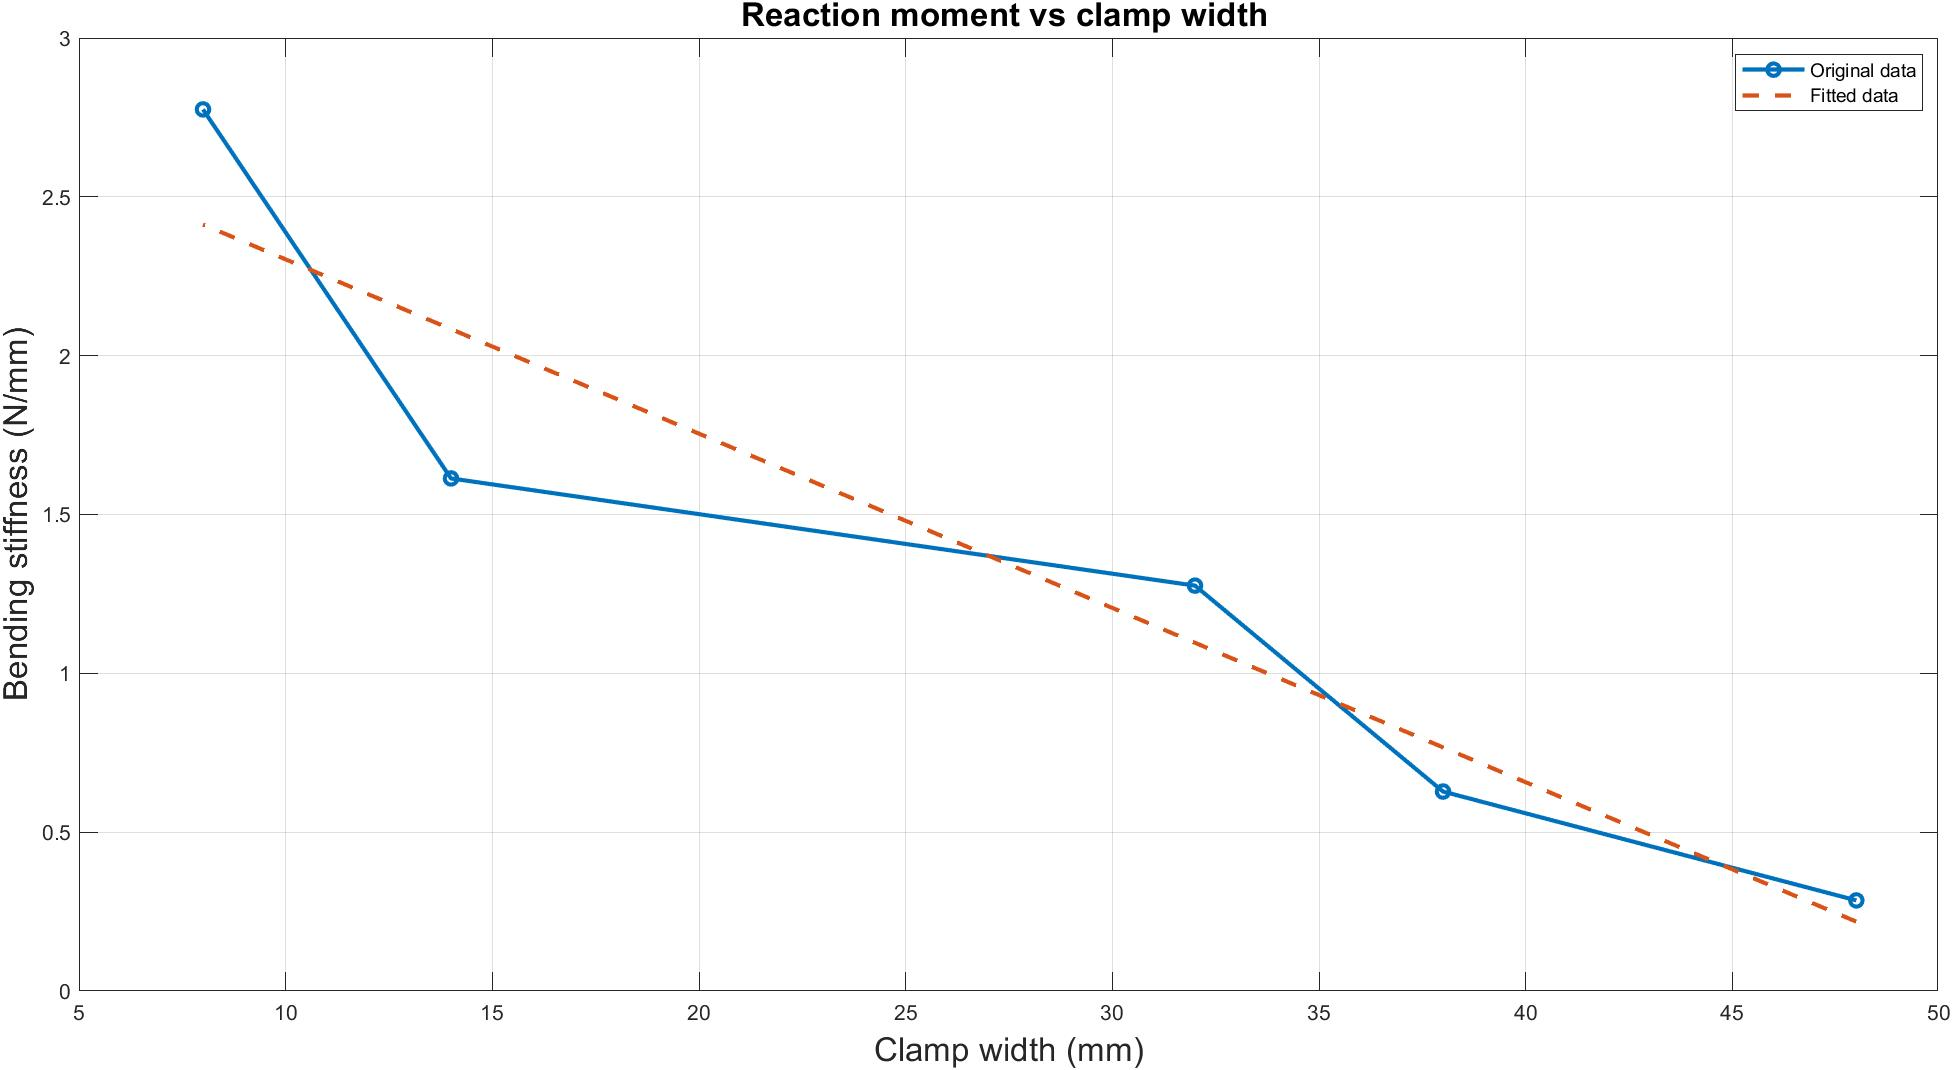
\includegraphics[width=15cm]{images/bend_stiffness.jpg}
    \caption{Bending stiffness plotted against clamp width}
    \label{fig:bendstiff}
\end{figure}
Plot \ref{fig:bendstiff} establishes the bending stiffness against clamp width and it can be seen that the bending stiffness varies almost linearly with the bending stiffness. The equation showing the following linear fit is given by equation \ref{eq:bendstiff} which is the same as equation \ref{eq:maxRM}. 
\begin{equation}
     K=-2.87\times W+ 164.24
     \label{eq:bendstiff}
 \end{equation}
 